\documentclass{beamer}
\usetheme{Boadilla}
\usepackage{graphicx}
\title{Predicting NHL Team Success}
\author{Eric Foote}
\institute{UNBSJ}
\date{December 4 2018}

\begin{document}

	\begin{frame}
		\titlepage
	\end{frame}
\begin{frame}
\begin{itemize}
	\frametitle{Overview}
	\item In this discussion I use multiple linear and ridge regression techniques to predict National Hockey Leauge(NHL) team points for the previous season of 2017-2018 as a method to predict overall team success. 
	\item I also use logistic regression to predict the probability that a team makes the playoffs
\end{itemize}
\end{frame}
\begin{frame}
	\begin{itemize}
		\frametitle{What we are going to Discuss}
	\item We are first going to talk about the dataset used
	\item Then we are going to talk about the theory behind each of the models
	\item Then the implementation of the models
	\item Finally the results
	\end{itemize}
\end{frame}
\begin{frame}
	\frametitle{Dataset}
	\begin{itemize}
	\item How we got the data?
	\item What variables were removed?	
	\item What variables were created?
	\item What are we going to consider for variables?
	\end{itemize}
\end{frame}
\begin{frame}
	\frametitle{How we got Data?}
	\begin{itemize}
	\item Comes from the NHL Stats application programmer interface(API)
	\item https://statsapi.web.nhl.com/api/v1
	\item Make API calls using the RJSON package in R
	\item /teams/i/stats?season=20072008 where i is the unique team id
	\item Each call creates a data frame that needs to be cleaned
	\end{itemize}
\end{frame}
\begin{frame}
	\frametitle{Data Cleaning}
	\begin{itemize}
	\item $\$$stats[[1]]$\$$splits[[1]] extracts the variables that we need
	\item The 2012-2013 season was removed due to the 48 game season
	\item Check for highly corrleated variables
	\end{itemize}
\end{frame}
\begin{frame}
	\frametitle{Correlation Matrix}
\begin{figure}
\centering
\includegraphics[width=0.7\linewidth]{"Correlation Matrix 1"}
\caption{1}
\label{fig:correlation-matrix-1}
\end{figure}
\end{frame}
\begin{frame}
\begin{figure}
	\centering
	\includegraphics[width=0.7\linewidth]{"Correlation Matrix 2"}
	\caption{2}
	\label{fig:correlation-matrix-2}
\end{figure}
\end{frame}
\begin{frame}
\begin{figure}
	\centering
	\includegraphics[width=0.7\linewidth]{"Correlation Matrix 3"}
	\caption{3}
	\label{fig:correlation-matrix-3}
\end{figure}
\end{frame}
\begin{frame}
\begin{figure}
	\centering
	\includegraphics[width=0.7\linewidth]{"Correlation Matrix 4"}
	\caption{4}
	\label{fig:correlation-matrix-4}
\end{figure}
\end{frame}
\begin{frame}
\begin{figure}
	\centering
	\includegraphics[width=0.7\linewidth]{"Correlation Matrix 5"}
	\caption{5}
	\label{fig:correlation-matrix-5}
\end{figure}
\end{frame}
\begin{frame}
\begin{figure}
	\centering
	\includegraphics[width=0.7\linewidth]{"Correlation Matrix 6"}
	\caption{6}
	\label{fig:correlation-matrix-6}
\end{figure}
\end{frame}
\begin{frame}
	\frametitle{What does this tell us?}
	\begin{itemize}
		\item Our predictor points is nearly perfectly correlated with wins, losses and point percentage
		\item So we remove them
		\item over time losses are also removed since they are in points calculation
		\item faceOff losses are also removed since faceOff wins are in the set
	\end{itemize}
\end{frame}
\begin{frame}
\frametitle{Dataset Description}
	\begin{itemize}
	\item 270 observations to build model
	\item 2007-2008 until 2016-2017 
	\item 24 variables
	\end{itemize}
\end{frame}
\begin{frame}
	\frametitle{Variables considered}
	\begin{itemize}
		\item Points: a team gets 2 for a win and 1 for a overtime loss
		\item Goals per game: average number of goals a team scores per game
		\item Goals against per game: average number of goals a team gives up 
		\item evGAARatio: goals the goalie gives up per even strength regulation time
		\item Power play percentage: percentage of power play goals a team scores
		\item Power play goals: the number of Power play goals a team scores
	\end{itemize}
\end{frame}
	\begin{frame}
	\begin{itemize}
	\item Penalty kill percentage: percentage of power plays against that do not result in a goal
	\item Power play goals against: number of power play goals against
	\item Power play opportunities: number of power plays a team got during the season
	\item Shots per game: average number of shots on goal
	\item Shots allowed: average number of that a team gives up
\end{itemize}
\end{frame}
\begin{frame}
	\begin{itemize}
		\item Win score first: percentage of wins that a team scored first
		\item Win opponent scored first: percentage of wins that the opponent scored first
		\item Win leading after first period: percentage of wins that a team had the lead after the first period
		\item Win leading after second period: percentage of wins that a team had the lead after the second period
		\item Win out shooting opponent: percentage of wins that a team out shot the opponent
		\item Win out shot by opponent: percentage of wins that the opponent out shot the team
	\end{itemize}
\end{frame}
\begin{frame}
	\begin{itemize}
		\item Shooting percentage: percentage of shots that resulted in goals
		\item Save percentage: percentage of shots that did not result in goals against
		\item Face offs taken: number of face offs taken 
		\item Face offs won: number of face offs won
		\item Face off win percentage: percentage of face offs won
	\end{itemize}
\end{frame}
\begin{frame}
	\frametitle{Additional Variable Definition}
	\begin{itemize}
		\item made Playoffs
		\item We define this categorical variable ourselves 
		\item Definition: this variable gets a 1 if a team makes the playoffs and a 0 if a team misses the playoffs
	\end{itemize}
\end{frame}
\begin{frame}
\frametitle{Methods}
	\begin{itemize}
		\item Multiple Linear Regression
		\item AIC Variable Selection
		\item Ridge Regression
		\item Logistic Regression
	\end{itemize}
\end{frame}
\begin{frame}
\frametitle{Multiple Linear Regression}
	\begin{itemize}
	\item The multiple linear regression model expresses the mean of response variable $Y$ as a function of one or more distinct predictor variables $x_1,...,x_k$
	\begin{center}
		$\mu_{Y|_{x_1...x_k}} = \beta_0 + \beta_1x_1 + ...+ \beta_kx_k$
	\end{center} 
	\item Which can be rewritten as: 
	\begin{center}
		$Y|_{x_1...x_k} = \beta_0 + \beta_1x_1 + \beta_2x_2 + ... + \beta_kx_i + \epsilon_i$ where $i = 1,2,3,...,n$
	\end{center} 
	\item where $\beta_k$ are our model parameters and $\epsilon_i$ is the random difference between $Y|_{x_i}$ and its mean $\mu|_{x_i}$
	\end{itemize}
\end{frame}
\begin{frame}
\begin{itemize}
	\item We can express a series of the first equations in matrix form as
	\begin{center}$
		Y = \begin{bmatrix}
		Y_1 \\
		Y_2 \\
		... \\
		Y_n
		\end{bmatrix} \beta = \begin{bmatrix}
		\beta_0 \\
		\beta_1 \\
		... \\
		\beta_k
		\end{bmatrix} \epsilon = \begin{bmatrix}
		\epsilon_1 \\
		\epsilon_2 \\
		... \\
		\epsilon_k
		\end{bmatrix}$ 
		\end{center}
\begin{center}$
	x = \begin{bmatrix}
	1 & x_{11} & x_{21} & x_{31} & ... x_{k1} \\
	1 & x_{12} & x_{22} & x_{32} & ... x_{k2} \\
	... & ... & ... & ... & ... \\
	1 & x_{1n} & x_{2n} & x_{3n} & ... x_{kn} \\
	\end{bmatrix}
	$\end{center}
\end{itemize}
\end{frame}
\begin{frame}
\frametitle{Assumptions}
\begin{itemize}
\item E($\epsilon$) = $\hat{0}$ and $var(\epsilon)$ = $E(\epsilon * \epsilon^T) = \sigma^2 I$ \\
\item $\epsilon_i$ are independent $\forall i$ \\
\item Predictor variables are not highly correlated with each other 
\item The variance of error terms are similar across the values of independent variables
\end{itemize}
\end{frame}
\begin{frame}
\frametitle{AIC Variable Selection}
	\begin{itemize}
		\item The Akaike Information Criterion
		\item Select a model to balance accuracy and simplicity
		\begin{center}$
			AIC_p = nln(\frac{SSE_p}{n}) + 2p	
		$\end{center}
		\item An advantage to AIC is it allows us to compare non-nested models
		\item A model is nested if "the parameters in one model are a subset of another"
	\end{itemize}
\end{frame}
\begin{frame}
\frametitle{Ridge Regression}
	\begin{itemize}
		\item Alternative estimation method that may be used to advantage when the predictor variables are highly collinear
		\item This helps us since some of our variables are computed from one another 
		\item The first thing we need to define is the ridge estimators which have been described by Hoerl and Kennard in the 1970's as a class of estimators indexed by a parameter $K \geq 0$. The estimator is
		\begin{center}$
			\hat{\theta}(k) = (Z^TZ + kI)^{-1}Z^TY 
			$\end{center}
	\end{itemize}
\end{frame}
\begin{frame}
	\begin{itemize}
		\item The idea of ridge regression is to pick a value of $k$ for which the reduction in total variance is not exceeded by the increase in bias. 
		\item Usually a value of $k$ is chosen by computing $\hat{\theta}_1,...,\hat{\theta}_p$ for a range of $k$ values between 0 and 1 and plotting the results against $k$. 
		\item This graph is known as the ridge trace and is used to select an appropriate value for k.
		\item In R this graph is plotted against $ln(k)$
		\item \url{https://ncss-wpengine.netdna-ssl.com/wp-content/themes/ncss/pdf/Procedures/NCSS/Ridge_Regression.pdf}
	\end{itemize}
\end{frame}
\begin{frame}
	\begin{itemize}
		\item If we have the standard form of a regression equation:
		\begin{center}$
			\hat{Y}	= \theta_1\hat{X}_1 + \theta_2\hat{X}_2 + ... + \theta_p\hat{X}_p
			$\end{center}
		\item The equations used for estimating the ridge regression coefficients are
		\begin{center}
			$(1+k)\theta_1 + r_{12}\theta_2 + ... + r_{1p}\theta_p = r_{1y} \\
			r_{21}\theta_1 + (1+k)\theta_2 + ... + r_{2p}\theta_p = r_{2y} \\
			r_{p1}\theta_1 + r_{p2}\theta_2 + ... + (1+k) = r_{py}$
		\end{center}
	\item This is the alternate method to find them
	\item where $r_{ij}$ is the correlation between the ith and jth predictor variables and $r_{iy}$ is the correlation between the ith predictor variable and the response variable $\hat{Y}$
	\end{itemize}
\end{frame}
\begin{frame}
	\frametitle{Assumptions}
	\begin{itemize}
		\item Same as Multiple Linear Regression
		\item E($\epsilon$) = $\hat{0}$ and $var(\epsilon)$ = $E(\epsilon * \epsilon^T) = \sigma^2 I$ 
		\item $\epsilon_i$ are independent $\forall i$ 
		\item Predictor variables are not highly correlated with each other 
		\item The variance of error terms are similar across the values of independent variables
	\end{itemize}
\end{frame}
	\begin{frame}
		\frametitle{Logistic Regression}
		\begin{itemize}
		\item Response variable is qualitative	
		\item logistic model can be expressed in the general form as: 
		\begin{center}$
			P(Y=1|X_1 = x_1, ..., X_p = x_p) = \frac{e^{(\beta_0 + \beta_1x_1 + \beta_2x_2 + ... + \beta_kx_k)}}{1 + e^{(\beta_0 + \beta_1x_1 + \beta_2x_2 + ... + \beta_kx_k)}}
		$\end{center}
		\end{itemize}
	\end{frame}
	\begin{frame}
		\frametitle{Assumptions}
		\begin{itemize}
			\item \url{https://www.statisticssolutions.com/assumptions-of-logistic-regression/}
			\item Does not require any of the previous assumptions
			\item Requires a binary dependent variable
			\item Observations need to be independent of each other 
			\item Requires little or no multicollinearity 
			\item Independent variables need to be linearly related to log odds
			\item Large sample size
		\end{itemize}
	\end{frame}
\begin{frame}
	\frametitle{Results}
	\begin{itemize}
		\item We are going to break it up into 3 sections
		\item Multiple linear regression
		\item Ridge regression
		\item Logistic regression
	\end{itemize}
\end{frame}
\begin{frame}
\frametitle{Results for Multiple Linear Regression}
\begin{itemize}
	\item Two different techniques for variable selection
	\item AIC on the model containing every variable to reduce it to a better model 
	\item $R^2$ values from the full model to create a smaller model
\end{itemize}
\end{frame}
\begin{frame}
\frametitle{AIC Results}
\begin{itemize}
	\item the AIC model is: 
	\begin{center}$
		points = 11.8895(goalsPerGame) - 14.2963(goalsAgainstPerGame) + 0.1168(powerPlayPercentage) + 24.9296(winScoreFirst) + 26.3916(winOppScoreFirst) - 10.1651(winLeadSecondPer) + 24.6731(winOutshootOpp) + 23.2772(winOutshotByOpp) + 0.1465(faceOffWinPercentage) + 48.08239  
		$\end{center}
\end{itemize}
\end{frame}
\begin{frame}
\begin{itemize}
	\begin{figure}
		\centering
		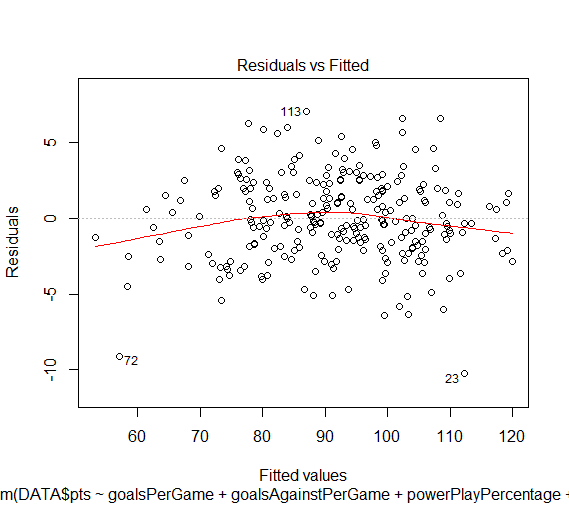
\includegraphics[width=0.7\linewidth]{AIC1}
		\caption{Residuals vs Fitted Values for AIC}
		\label{fig:Residuals vs Fitted Values for AIC}
	\end{figure}
\end{itemize}
\end{frame}
\begin{frame}
	\begin{figure}
		\centering
		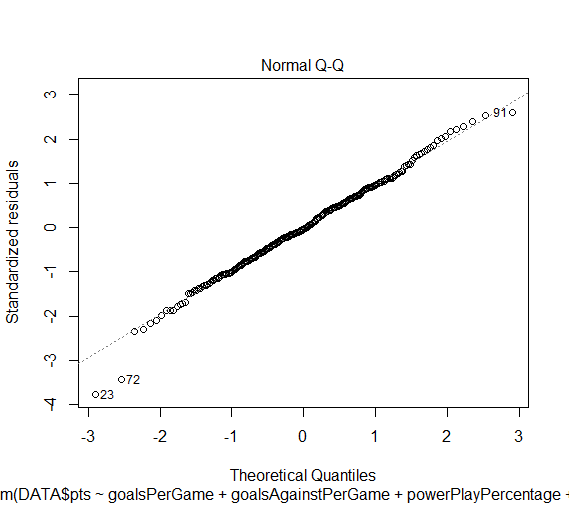
\includegraphics[width=0.7\linewidth]{AIC2}
		\caption{QQ Plot for AIC}
		\label{fig:QQ Plot for AIC}
	\end{figure}
\end{frame}
\begin{frame}
	\begin{figure}
		\centering
		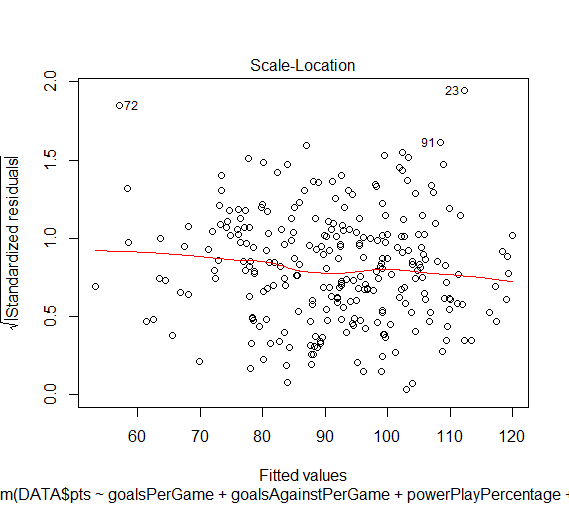
\includegraphics[width=0.7\linewidth]{AIC3}
		\caption{Scale-Location for AIC}
		\label{fig:Scale-Location for AIC}
	\end{figure}
\end{frame}
\begin{frame}
	\begin{figure}
		\centering
		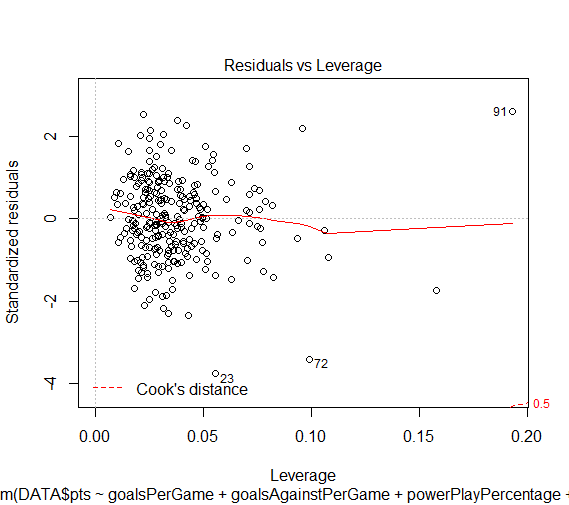
\includegraphics[width=0.7\linewidth]{AIC4}
		\caption{Residuals vs Leverage for AIC}
		\label{fig:Residuals vs Leverage for AIC}
	\end{figure}
\end{frame}
\begin{frame}
	\begin{itemize}
	\begin{figure}
	\centering
	\includegraphics[width=0.7\linewidth]{"AIC Prediction"}
	\caption{AIC Prediction}
	\label{fig:AIC Prediction}
\end{figure}	
	\end{itemize}
\end{frame}
\begin{frame}
\frametitle{$R^2$ Results}
\begin{itemize}
	\item $R^2$ Model is:
	\begin{center}$
		points = 35.603(winScoreFirst) + 36.087(winOppScoreFirst) + 44.795(winOutshootOpp) + 42.294(winOutshotByOpp) + 12.525  
		$\end{center}
\end{itemize}
\end{frame}
\begin{frame}
	\begin{itemize}
		\begin{figure}
			\centering
			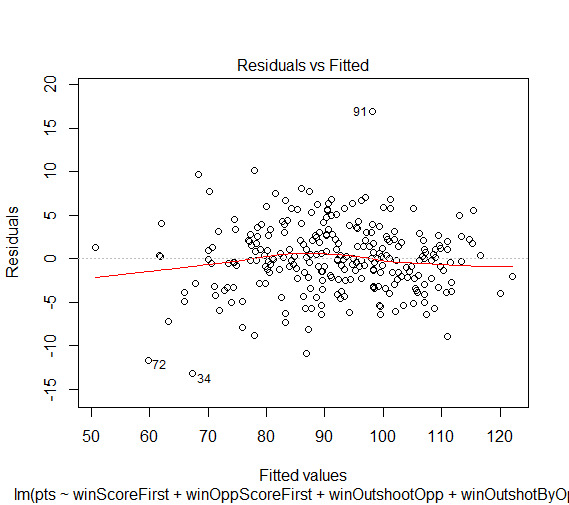
\includegraphics[width=0.7\linewidth]{R1}
			\caption{Residuals vs Fitted Values for R Squared}
			\label{fig:Residuals vs Fitted Values for R Squared}
		\end{figure}
	\end{itemize}
\end{frame}
\begin{frame}
	\begin{figure}
		\centering
		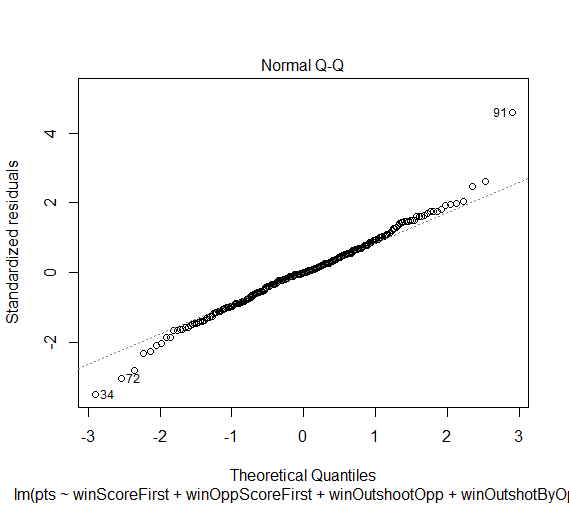
\includegraphics[width=0.7\linewidth]{R2}
		\caption{QQ Plot for R Squared}
		\label{fig:QQ Plot for R Squared}
	\end{figure}
\end{frame}
\begin{frame}
	\begin{figure}
		\centering
		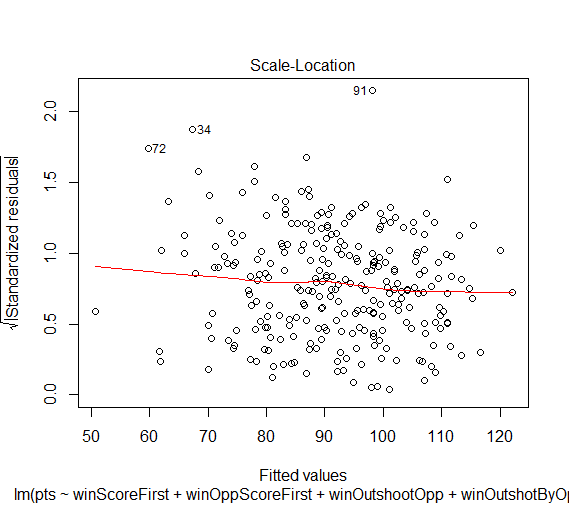
\includegraphics[width=0.7\linewidth]{R3}
		\caption{Scale-Location for R Squared}
		\label{fig:Scale-Location for R Squared}
	\end{figure}
\end{frame}
\begin{frame}
	\begin{figure}
		\centering
		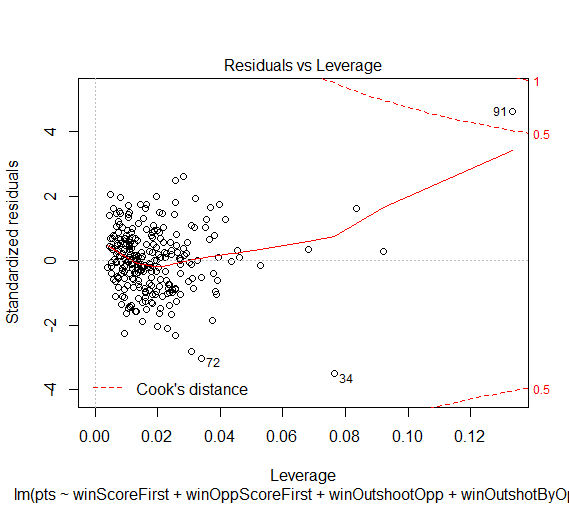
\includegraphics[width=0.7\linewidth]{R4}
		\caption{Residuals vs Leverage for R Squared}
		\label{fig:Residuals vs Leverage for R Squared}
	\end{figure}
\end{frame}
\begin{frame}
	\begin{figure}
		\centering
		\includegraphics[width=0.7\linewidth]{"R Prediction"}
		\caption{R Prediction}
		\label{fig:R Prediction}
	\end{figure}	
\end{frame}
\begin{frame}
\frametitle{Errors}
	\begin{itemize}
		\item What is the Error in our estimation?
		\begin{center}
			$Error = |Actual - Theoritical|$
		\end{center}
	\end{itemize}
\end{frame}
\begin{frame}
\frametitle{AIC Error}
	\begin{figure}
		\centering
		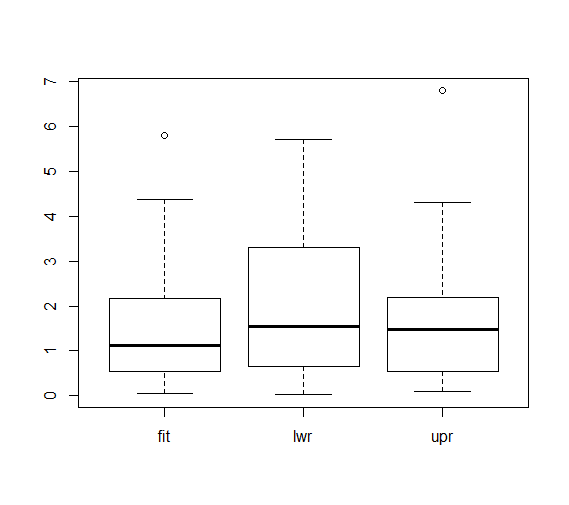
\includegraphics[width=0.7\linewidth]{AICPredictionError}
		\caption{AIC Error Plot}
		\label{fig:aicpredictionerror}
	\end{figure}
\end{frame}
\begin{frame}
	\frametitle{$R^2$ Error}
	\begin{figure}
		\centering
		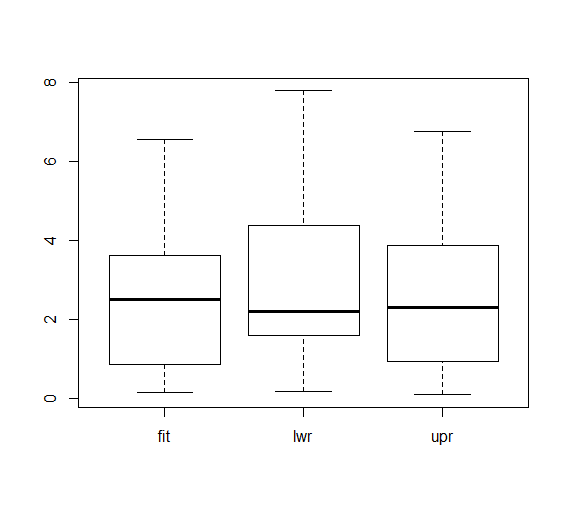
\includegraphics[width=0.7\linewidth]{RSquaredError}
		\caption{$R^2$ Error Plot}
		\label{fig:rsquarederror}
	\end{figure}
\end{frame}
\begin{frame}
	\begin{itemize}
		\item For the AIC model a majority of the predictions were one to two points off the actual value
		\item Most extreme case is the Los Angeles Kings which were five points off what they actually had. \item One reason for this is that LA had the lowest goals against per game in the NHL during this season at 2.890 goals against
		\item In the model we have $- 14.2963(goalsAgainstPerGame)$ 
		\item Another reason is that LA was ninth in wins when the opponent scored first at 0.4 or 40\% which is another variable with a heavy weight in our regression equation. 
	\end{itemize}
\end{frame}
\begin{frame}
	\begin{itemize}
		\item The second most extreme case is the Nashville Predators which were four points off their actual value 
		\item One reason for this is like LA they were second in goals against per game at 2.488. 
		\item 7th in wins when the team scored first
		\item We can draw the conclusion that good defensive teams that limit their goals against tend to have more points in this model. 
	\end{itemize}
\end{frame}
\begin{frame}
\begin{itemize}
	\item For the $R^2$ model a majority of estimates were off significantly
	\item Up to almost 4 points 
	\item This model also rewards teams for having lots of shots. 
	\item For example, the Boston Bruins were first in wins when the opponent scored first and third in wins when you out shoot the opponent, this increased the value of their prediction.
\end{itemize}
\end{frame}
\begin{frame}
	\frametitle{Ridge Regression}
\begin{itemize}
	\item R calculated 99 different $k$ values(or $\lambda$ as R calls it) and fit all 24 variables to it. \item This created the ridge trace
\end{itemize}	
\end{frame}
\begin{frame}
	\begin{figure}
		\centering
		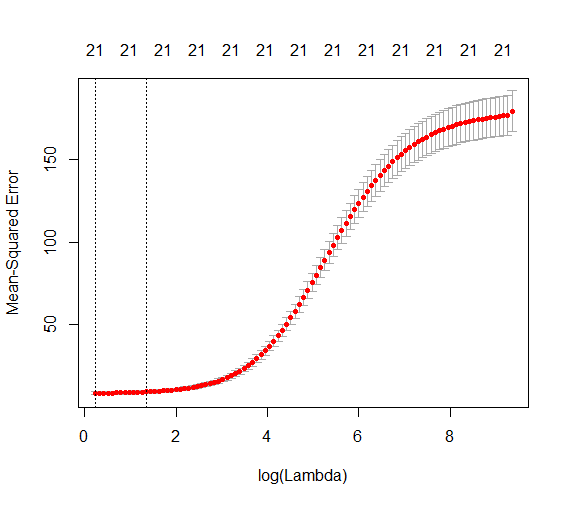
\includegraphics[width=0.7\linewidth]{RidgeTrace}
		\caption{Ridge Trace}
		\label{fig:ridgetrace}
	\end{figure}
\end{frame}
\begin{frame}
	\begin{figure}
		\centering
		\includegraphics[width=0.7\linewidth]{"Ridge Prediction"}
		\caption{Ridge Prediction}
		\label{fig:Ridge Prediction}
	\end{figure}
\end{frame}
\begin{frame}
	\begin{figure}
		\centering
		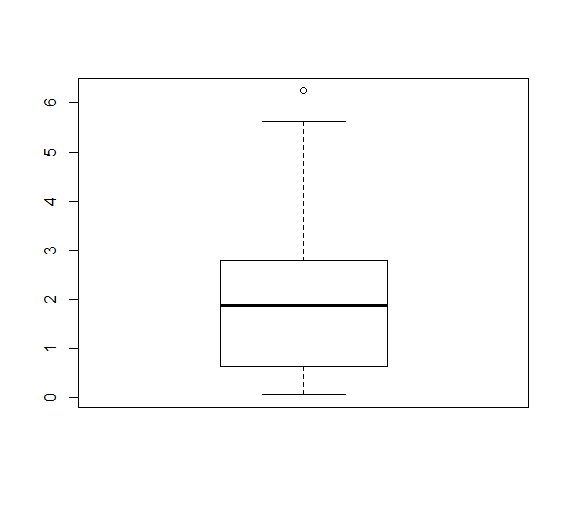
\includegraphics[width=0.7\linewidth]{RidgePredictionError}
		\caption{Ridge Prediction Error}
		\label{fig:ridgepredictionerror}
	\end{figure}
\end{frame}
\begin{frame}
	\begin{itemize}
		\item The most extreme error in this model is the Nashville Predators
		\item 6 points off their actual point value
		\item Since the ridge regression model takes every variable in our data set, it is simply due to them being in the top 15 for almost every variable in our set
	\end{itemize}
\end{frame}
\begin{frame}
	\frametitle{Logistic Regression}
	\begin{itemize}
		\item We are predicting the probability that a team makes the playoffs. 
		\item For this model we are strictly using every variable, rather than using AIC. 
		\item The model has these coefficients
		\begin{center}$
			madePlayoffs = -596.2016 + 0.6785186(pts) + 17.31825(goalsPerGame) - 6.797520(goalsAgainstPerGame) - 18.07236(evGAARatio) - 0.1268944(powerPlayPercentage) - 0.03467402(powerPlayGoals) - 0.1270233(powerPlayGoalsAgainst) - 0.004215109(powerPlayOpportunities) - 0.04239098(penaltyKillPercentage) - 0.3554432(shotsPerGame) - 16.05426(winLeadFirstPer) + 3.368749(winLeadSecondPer) + 3.367920(winOutshootOpp) + 12.48498(winOutshotByOpp) + 0.07043268(faceOffsTaken) - 0.1464181(faceOffsWon) + 7.594018(faceOffWinPercentage) - 1.656188(shootingPctg) + 214.9347(savePctg)   
			$\end{center}
	\end{itemize}
\end{frame}
\begin{frame}
\begin{figure}
	\centering
	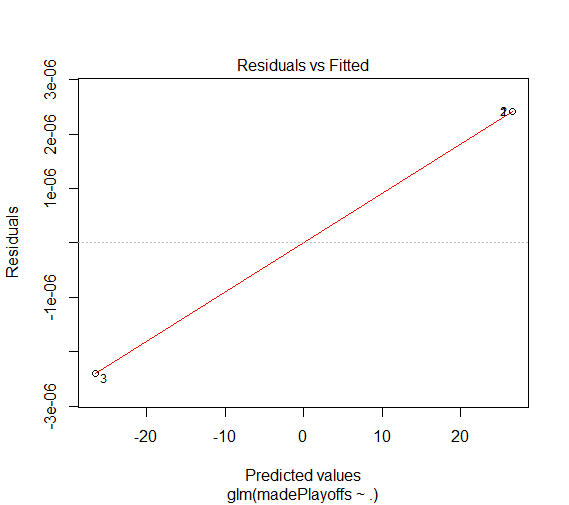
\includegraphics[width=0.7\linewidth]{Log1}
	\caption{Residuals vs Fitted Values for Logistic Regression}
	\label{fig:Residuals vs Fitted Values for Logistic Regression}
\end{figure}
\end{frame}
\begin{frame}
	\begin{figure}
		\centering
		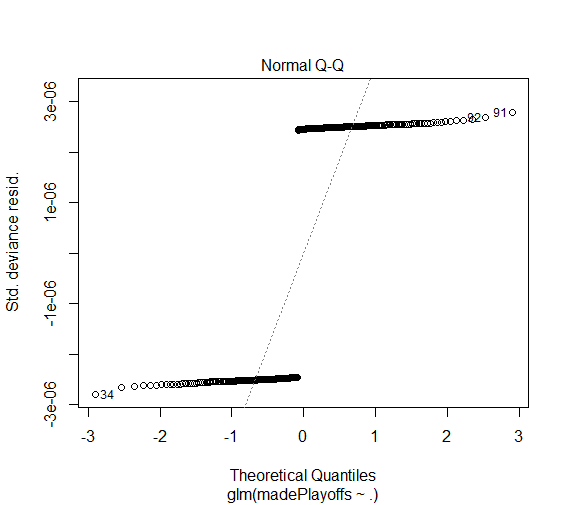
\includegraphics[width=0.7\linewidth]{Log2}
		\caption{QQ Plot for Logistic Regression}
		\label{fig:QQ Plot for R Squared}
	\end{figure}
\end{frame}
\begin{frame}
	\begin{figure}
		\centering
		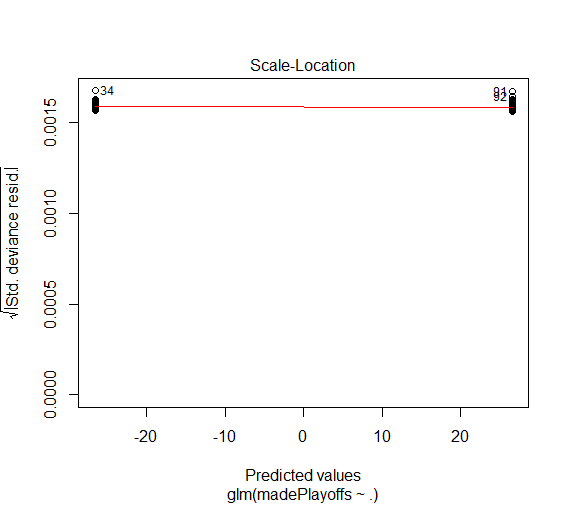
\includegraphics[width=0.7\linewidth]{Log3}
		\caption{Scale-Location for Logistic Regression}
		\label{fig:Scale-Location for Logistic Regression}
	\end{figure}
\end{frame}
\begin{frame}
	\begin{figure}
		\centering
		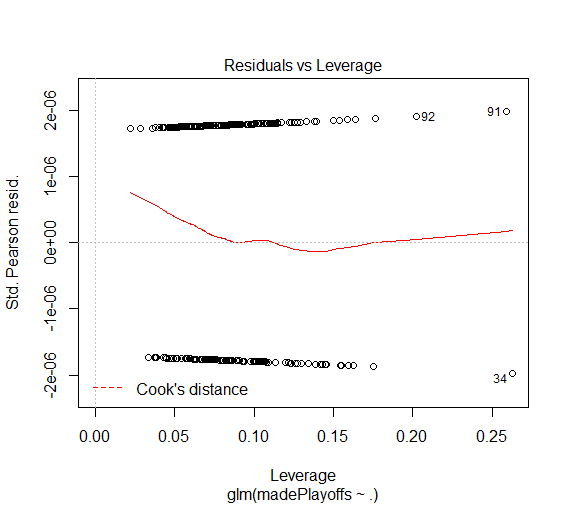
\includegraphics[width=0.7\linewidth]{Log4}
		\caption{Residuals vs Leverage for Logistic Regression}
		\label{fig:Residuals vs Leverage for Logistic Regression}
	\end{figure}
\end{frame}
\begin{frame}
	\begin{figure}
		\centering
		\includegraphics[width=0.7\linewidth]{"Logistic Prediction"}
		\caption{Logistic Prediction}
		\label{fig:Logistic Prediction}
	\end{figure}
\end{frame}
\begin{frame}
	\begin{itemize}
		\item This model has Anaheim, Boston, Vegas, Winnipeg, Washington, Toronto, Tampa Bay, San Jose, Philadelphia,Pittsburgh, New Jersey, Nashville, Minnesota, LA, Columbus and Dallas all having a high probability of making the playoffs.
		\item Only team out of this list that did not make the playoffs during this season was the Dallas, instead Colorado made it.
		\item One possible reason for this is during the 2013-2014 season the NHL changed the playoff format; rather then it being the top 8 teams from each conference making it; the top 3 teams from each division makes it and the two final teams representing each conference are wild card teams.
	\end{itemize}
\end{frame}
\begin{frame}
	\frametitle{Future Work}
	 \begin{itemize}
	 \item The next major step would be extend the models to predicting unknown or in progress years. 
	 \item I would also like to consider other variables that are commonly used in other areas such as WAR, Corsi, etc... 
	 \item I would also like to consider other machine learning algorithms that are commonly used
	 \item I would also like to finish up the graph based regression models
	 \end{itemize}
\end{frame}
\begin{frame}
	\frametitle{Conclusions}
	\begin{itemize}
		\item In the AIC model, defensive statistics were weighted heavier then offensive ones. 
		\item The $R^2$ model weighted shots very heavily due to variable selection. 
		\item The ridge regression model weighted teams which were the top of every category very heavily. \item Finally the logistic regression model predicted every playoff team for the previous season, except for Colorado
	\end{itemize}
\end{frame}
\begin{frame}
\frametitle{Bibliography}
		Joshua Weissbock Forecasting Success in the
		National Hockey League using
		In-Game Statistics and Textual Data School of Electrical Engineering and Computer Science
		Faculty of Engineering
		University of Ottawa,  Ottawa, Canada, 2014
		{Drew Hynes, nhlapi, January 9,2018, https://gitlab.com/dword4/nhlapi.git}
		Micah Blake McCurdy,Hockey Viz 2018,http://hockeyviz.com/txt/preview1819,2018-2019 Regular Season Predictions
		https://www.nhl.com/fans/nhl-centennial
		NHL Standings Predictions: Offseason Edition,Larry Fisher , July 22,2018, https://thehockeywriters.com/nhl-standings-predictions-offseason-edition-2019/
\end{frame}
\begin{frame}
		The Magnus Prediction Models,Estimating Individual Impact on NHL 5v5 Shot Rates, September 24, 2018, Micah Blake McCurdy,http://hockeyviz.com/txt/magnusEV
		The Magnus Prediction Models,September 30, 2018, Micah Blake McCurdy,http://hockeyviz.com/txt/magnus
		Introduction to Probability and Statistics Principles and Applications for Engineering and the Computing Sciences,J.Susan Milton Jesse C. Arnold, McGraw Hill 2003.
		Regression Analysis by Example Fifth Edition,Samprit Chatterjee and Ali S. Hadi,Wiley Publication.
		Statistics Solutions 2018,https://www.statisticssolutions.com/assumptions-of-multiple-linear-regression
		Top 10 Machine Learning Algorithms,https://www.dezyre.com/article/top-10-machine-learning-algorithms/202,May 11, 2018
		The Analysis Factor. Karen-Grace Martin. What are nested models? 2017.https://www.theanalysisfactor.com/what-are-nested-models/
		https://www.statisticssolutions.com/multicollinearity/
		https://ncss-wpengine.netdna-ssl.com/wp-content/themes/ncss/pdf/Procedures/NCSS/Ridge Regression.pdf
		https://www.statisticssolutions.com/assumptions-of-logistic-regression/
\end{frame}
\end{document}